\section{Implementation}
\label{sec:impl}

\name is implemented as a shallow extension of GHC Haskell and runs on top of
Cassandra, an off-the-shelf eventually consistent distributed data (or backing)
store responsible for all data management issues (i.e., replication, fault
tolerance, availability, and convergence).  Template Haskell is used to
implement static contract classification, and proof obligations are discharged
with the help of the Z3~\cite{Z3} SMT solver. Figure~\ref{fig:impl_mod}
illustrates the overall system architecture.

\begin{figure}
\begin{center}
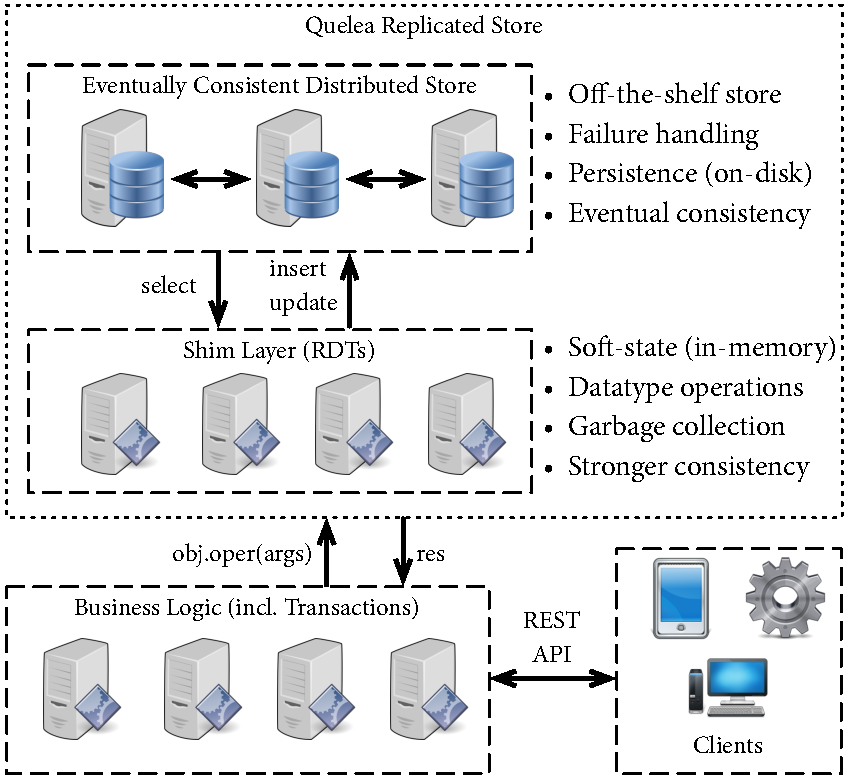
\includegraphics[width=\columnwidth]{Figures/ImplModel}
\end{center}
\caption{Implementation Model.}
\label{fig:impl_mod}
\end{figure}

Replicated data types and various consistency semantics are implemented and
enforced in the \emph{shim layer}. Our implementation supports eventual,
causal, and strong consistency for data type operations, and RC, MAV, and RR
semantics for transactions.  This functionality is implemented entirely on
top of the standard interface exposed by Cassandra. From an engineering
perspective, leveraging an off-the-shelf data store enables an
implementation comprising roughly only 2500 lines of Haskell code, which is
packaged as a library.

Each new effect in \name is realized as a row insertion in Cassandra, and
the state of an object is the set of all corresponding rows. The shim layer
maintains a causally consistent in-memory snapshot of a subset of objects in
the backing store, by explicitly tracking dependencies introduced between
effects due to visibility, session and same transaction
relations. Dependence tracking is similar to the techniques presented
in~\cite{BoltOn} and~\cite{Eiger}. Because Cassandra provides durability,
convergence, and fault tolerance, each shim layer node simply acts as a
soft-state cache, with no inter-node communication, and can safely be
terminated at any point. Similarly, new shim layer nodes can be spawned on
demand.

The shim layer nodes periodically fetch updates from the backing store for
eventually consistent operations, and on-demand for causally consistent and
strongly consistent operations. Strongly consistent operations are performed
after obtaining exclusive leases on objects. The lease mechanism is
implemented with the help of Cassandra's support for conditional updates and
expiring columns. Cassandra does not provide general-purpose
transactions. Since the transaction guarantees provided by \name are
coordination-free~\cite{BailisHAT}, we realize efficient implementations by
explicitly tracking dependencies between operations and transactions.
Importantly, the weaker isolation semantics of transactions in \name permit
transactions to be discharged if at least one shim layer node is reachable.

We utilize the \cf{summarize} function (\S~\ref{sec:summarize}) to summarize
the object state both in the shim layer node and the backing store, typically
when the number of effects on an object crosses a tunable threshold.
Shim layer summarization is straight-forward; a summarization thread takes the
local lock on the cached object, and replaces its state with the summarized
state. The shim layer node only remains unavailable for that particular object
during summarization (usually a few milliseconds). Performing summarization in
the backing store is more complicated since the whole process needs to be
atomic from a client's perspective, but Cassandra does not provide multi-row
transactions. We have engineered and implemented a scalable summarization
mechanism for the backing store that permits concurrent client operations, but
nonetheless prohibits these operations from witnessing intermediate states of
the summarization process.
